\chapter{Source Code}
%% Create a new environment for breaking code listings across pages.
%\newenvironment{longlisting}{\captionsetup{type=listing}}{}
%\begin{longlisting}
%	\caption{main zephyr}
%	\label{lst:zephyr}
%	\inputminted[bgcolor=LightGray,fontsize=\footnotesize,linenos]{c}{Figures/Code/main.c}
%\end{longlisting}

%\chapter{Timer Configurations}
%\begin{figure}[htbp]
%	\centering
%	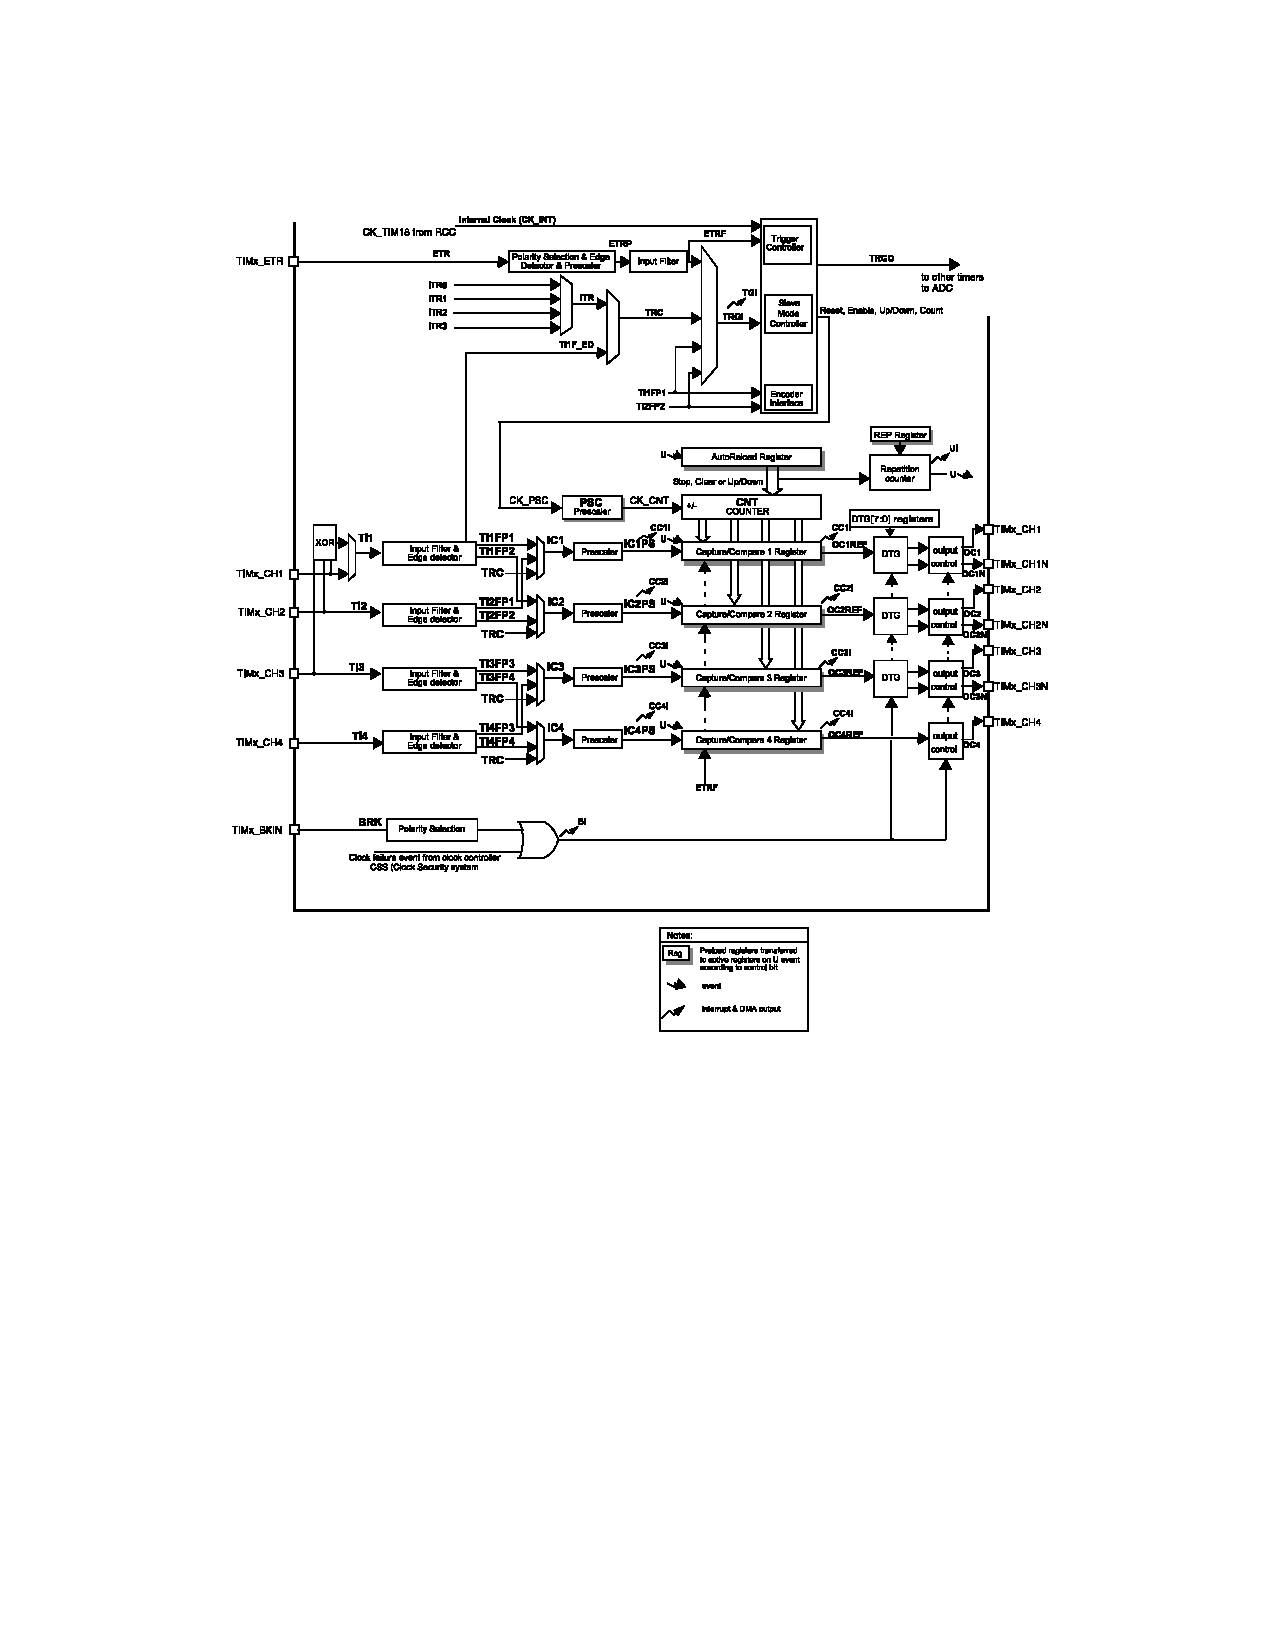
\includegraphics[width=.8\textwidth]{Figures/4_advanced_timer1_diagram.pdf}
%	\caption{Configuration of \texttt{TIMER1}}
%	\label{fig:4_timer1}
%\end{figure}
%\begin{figure}[htbp]
%	\centering
%	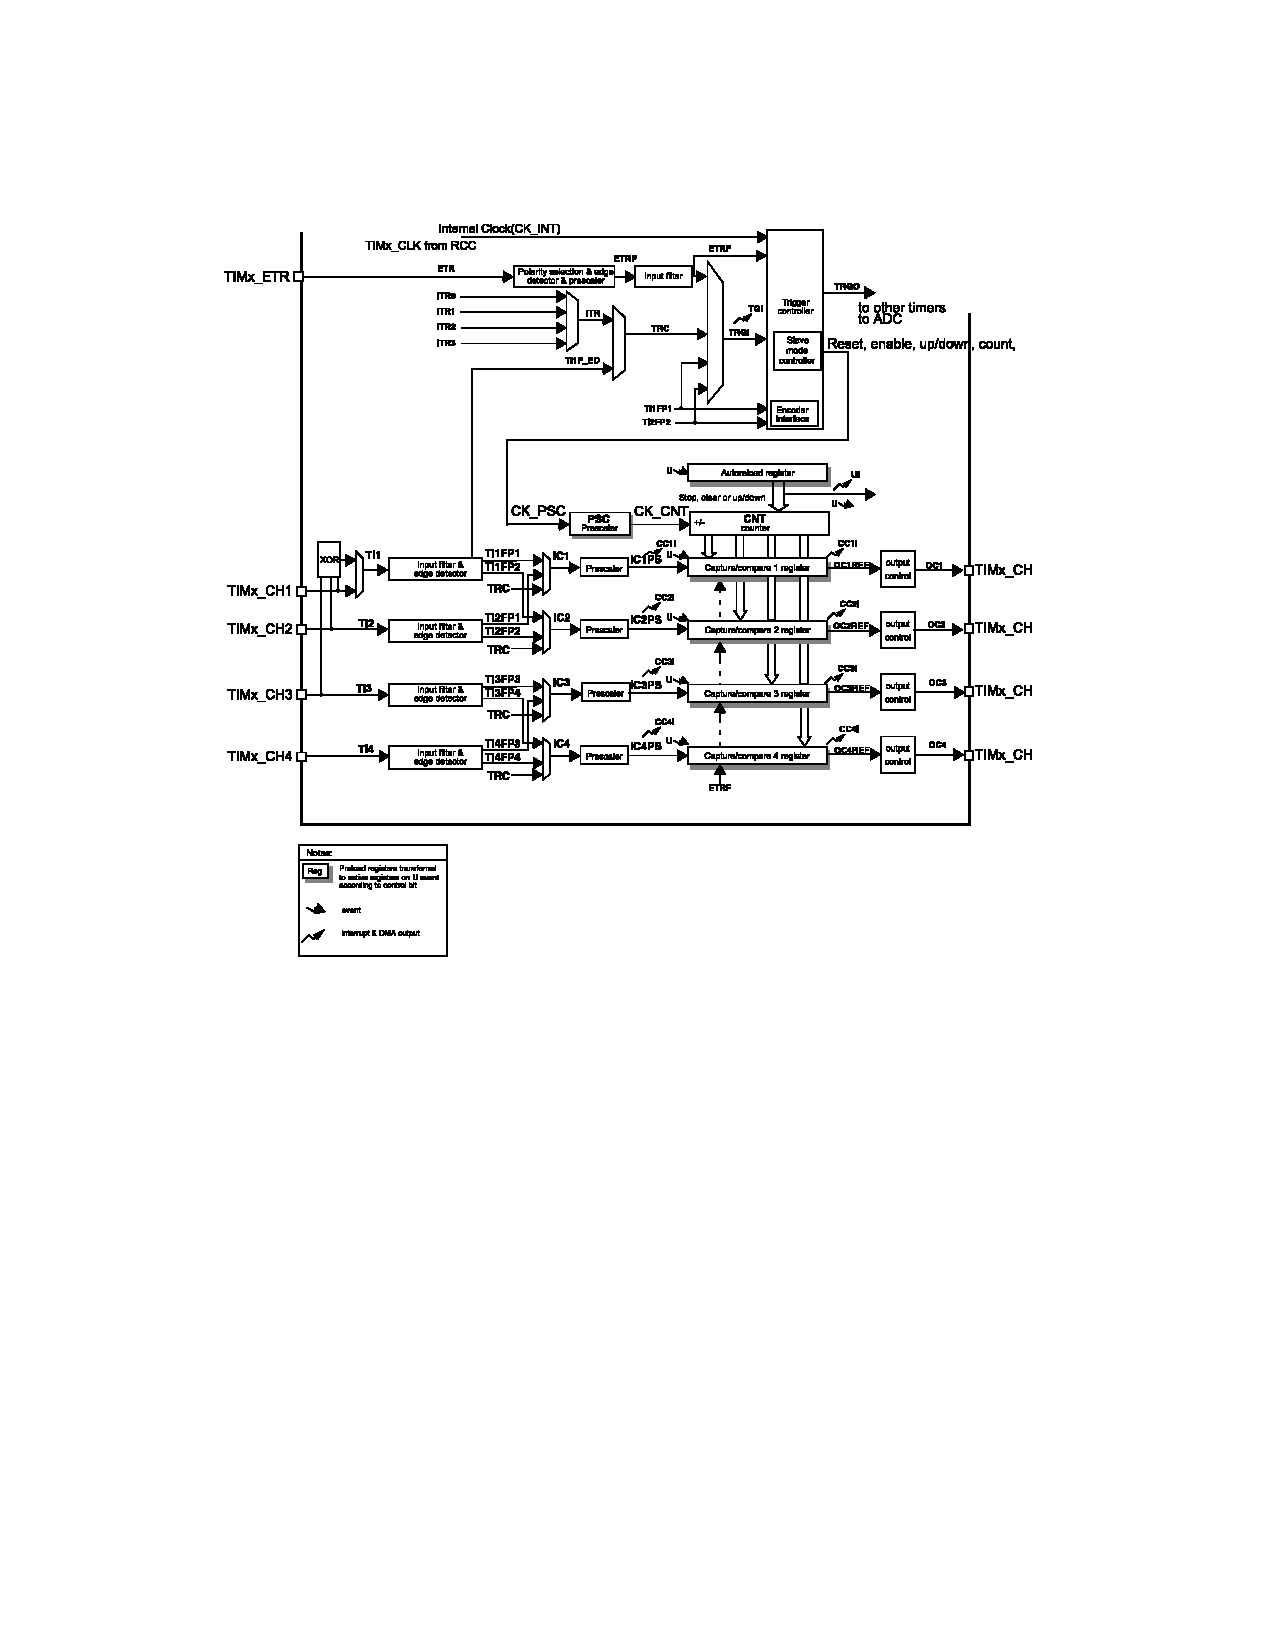
\includegraphics[width=.8\textwidth]{Figures/4_advanced_timer2-5_diagram.pdf}
%	\caption{Configuration of \texttt{TIMER2--5}}
%	\label{fig:4_timer2-5}
%\end{figure}
%\begin{figure}[htbp]
%	\centering
%	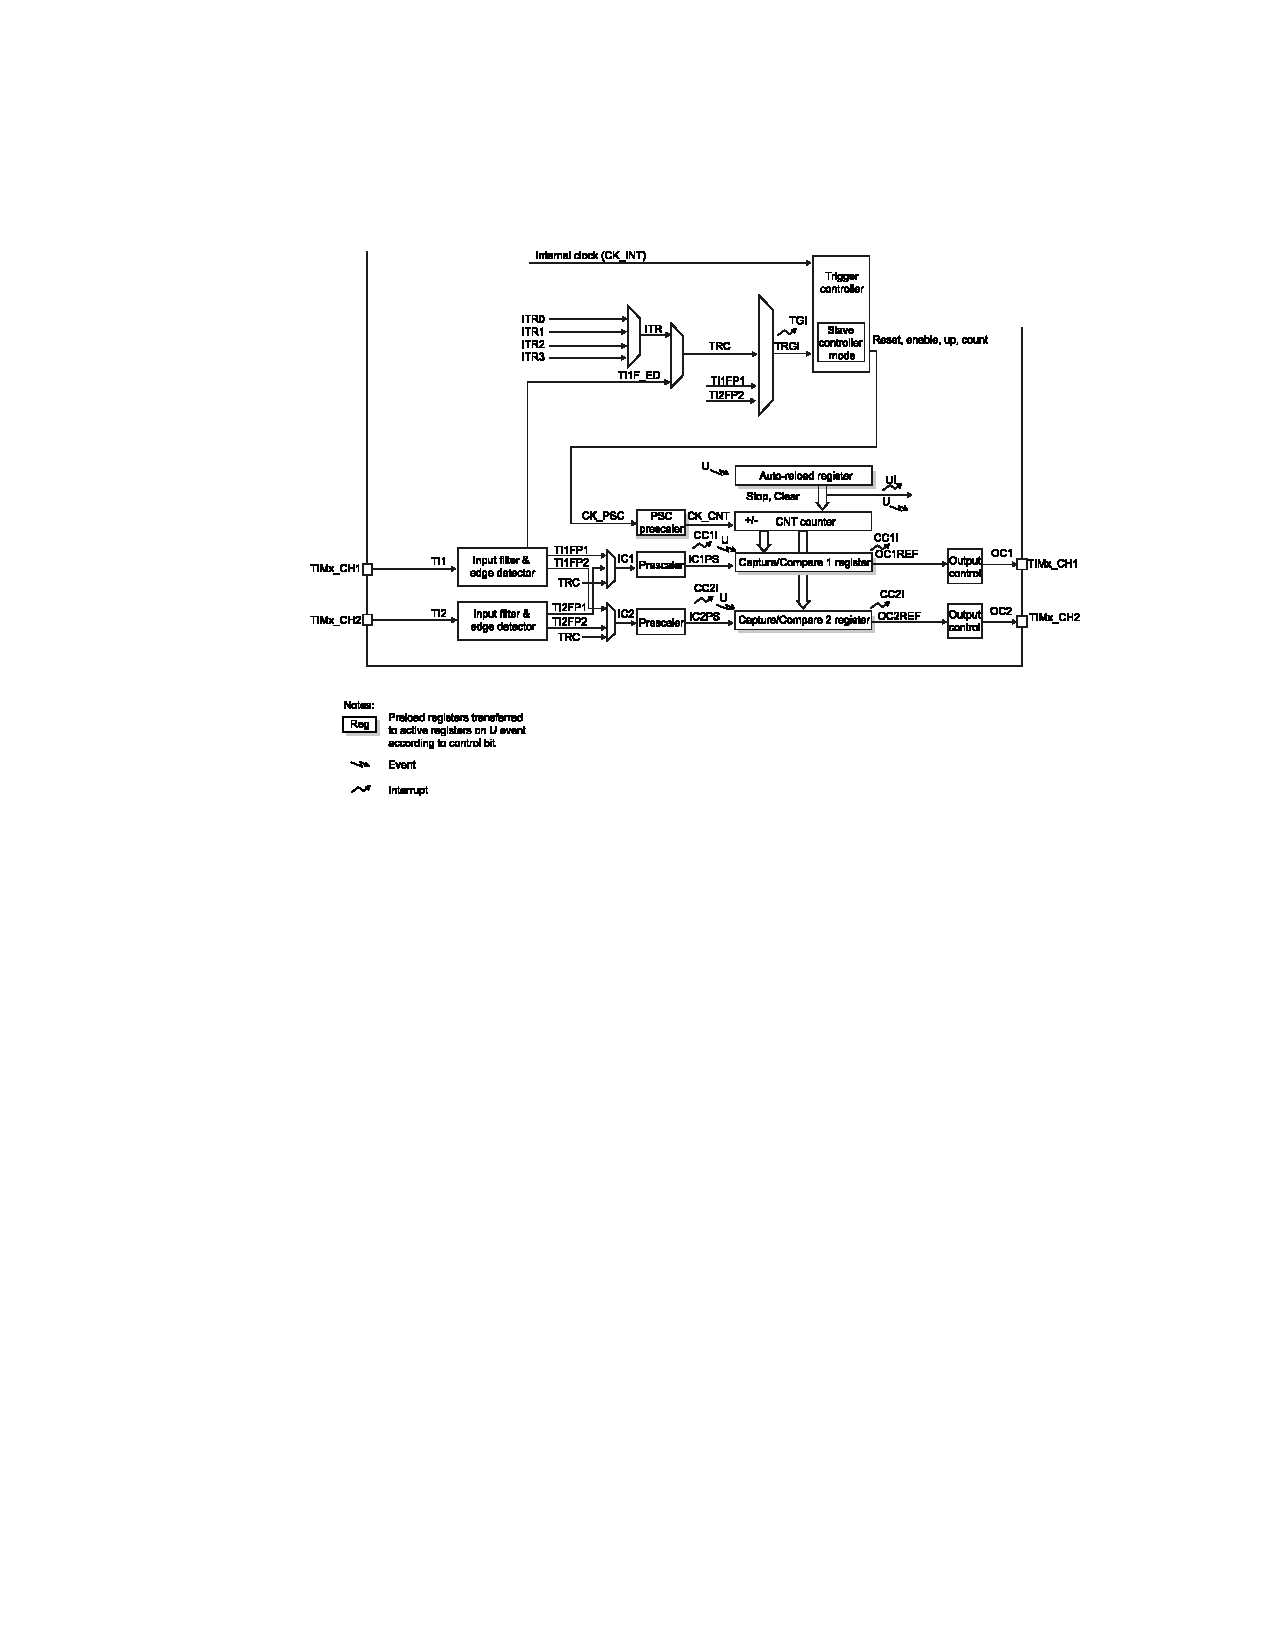
\includegraphics[width=.8\textwidth]{Figures/4_advanced_timer9_diagram.pdf}
%	\caption{Configuration of \texttt{TIMER9}}
%	\label{fig:4_timer9}
%\end{figure}

\chapter{Simulation Models}
\begin{figure}[htbp]
	\centering
	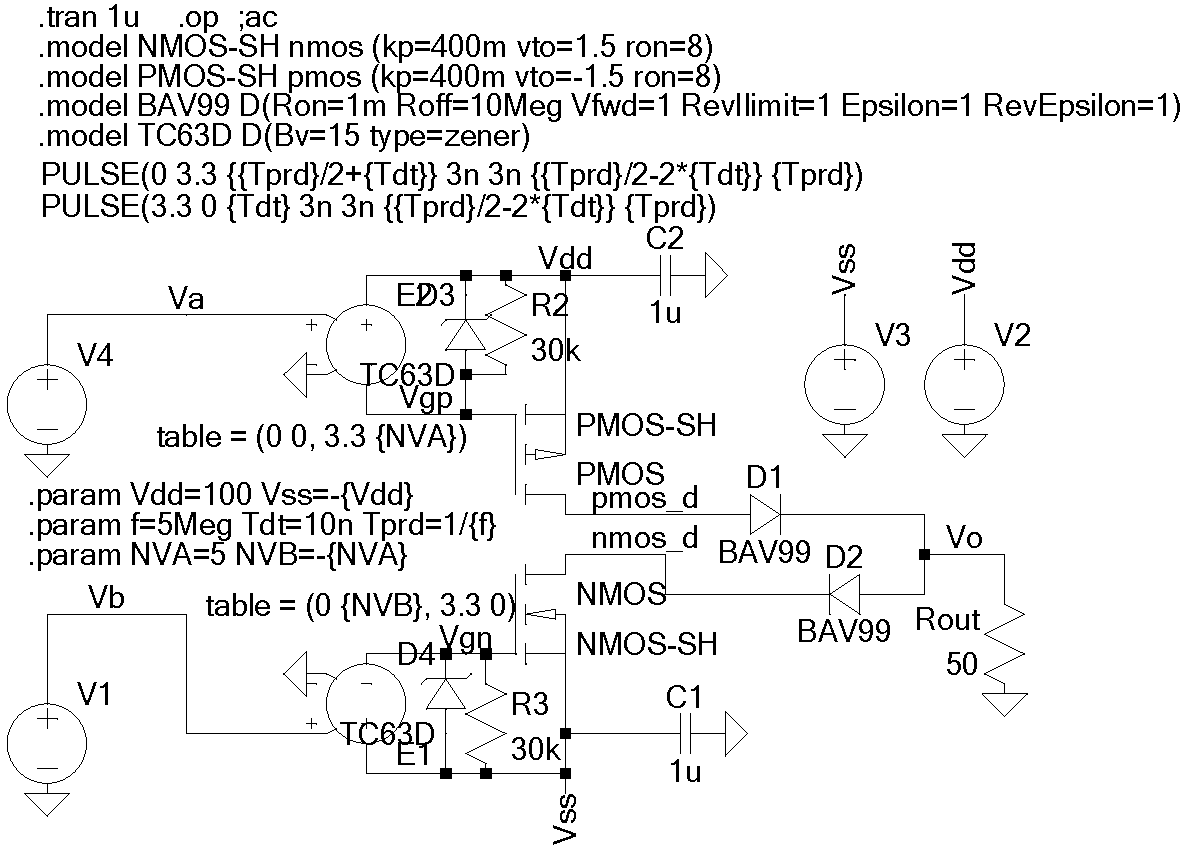
\includegraphics[width=.9\textwidth]{Figures/appendix/ltspice_transmitter.pdf}
	\caption{LTspice model of transmitter}
	\label{fig:app_ltspice_transmitter}
\end{figure}
\begin{figure}[htbp]
	\centering
	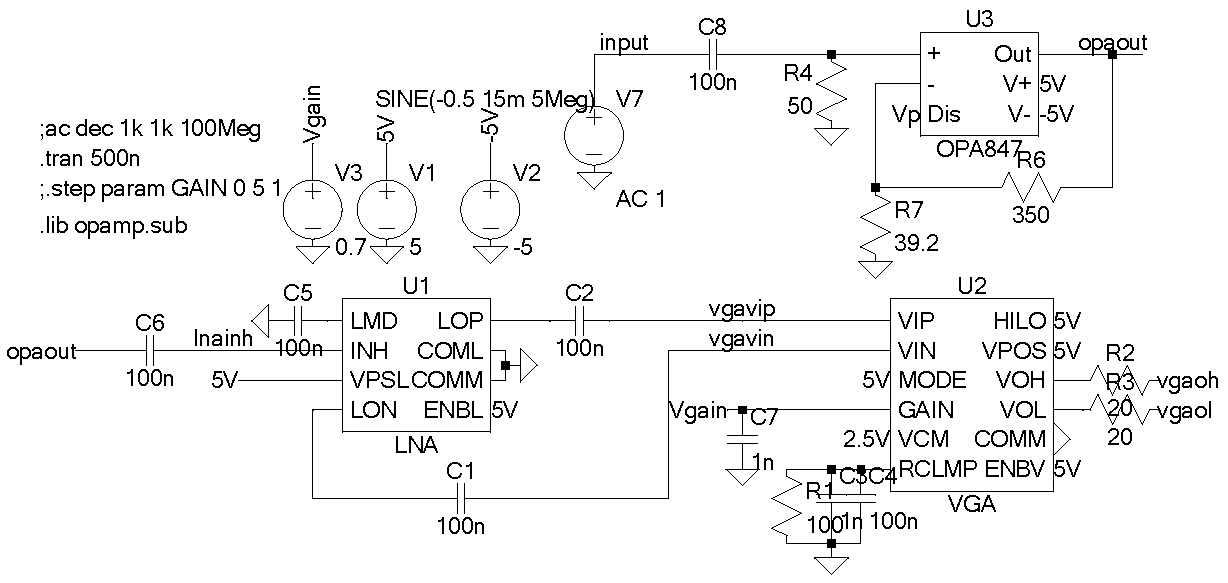
\includegraphics[width=.9\textwidth]{Figures/appendix/ltspice_preamp.pdf}
	\caption{LTspice model of preamplifier}
	\label{fig:app_ltspice_preamp}
\end{figure}
\begin{figure}[htbp]
	\centering
	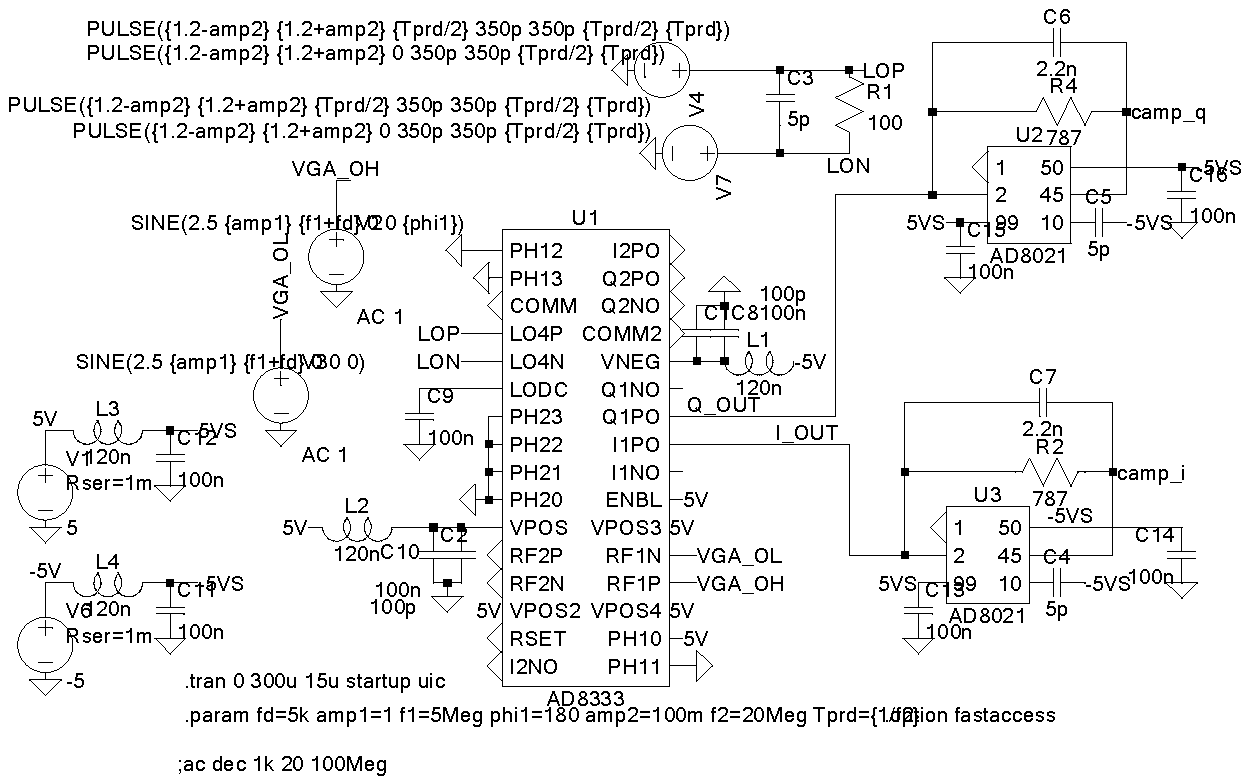
\includegraphics[width=.9\textwidth]{Figures/appendix/ltspice_demod.pdf}
	\caption{LTspice model of demodulator}
	\label{fig:app_ltspice_demod}
\end{figure}

%\chapter{Circuit Schematics}
%\begin{landscape}
%	\begin{figure}[htbp]
%		\centering
%		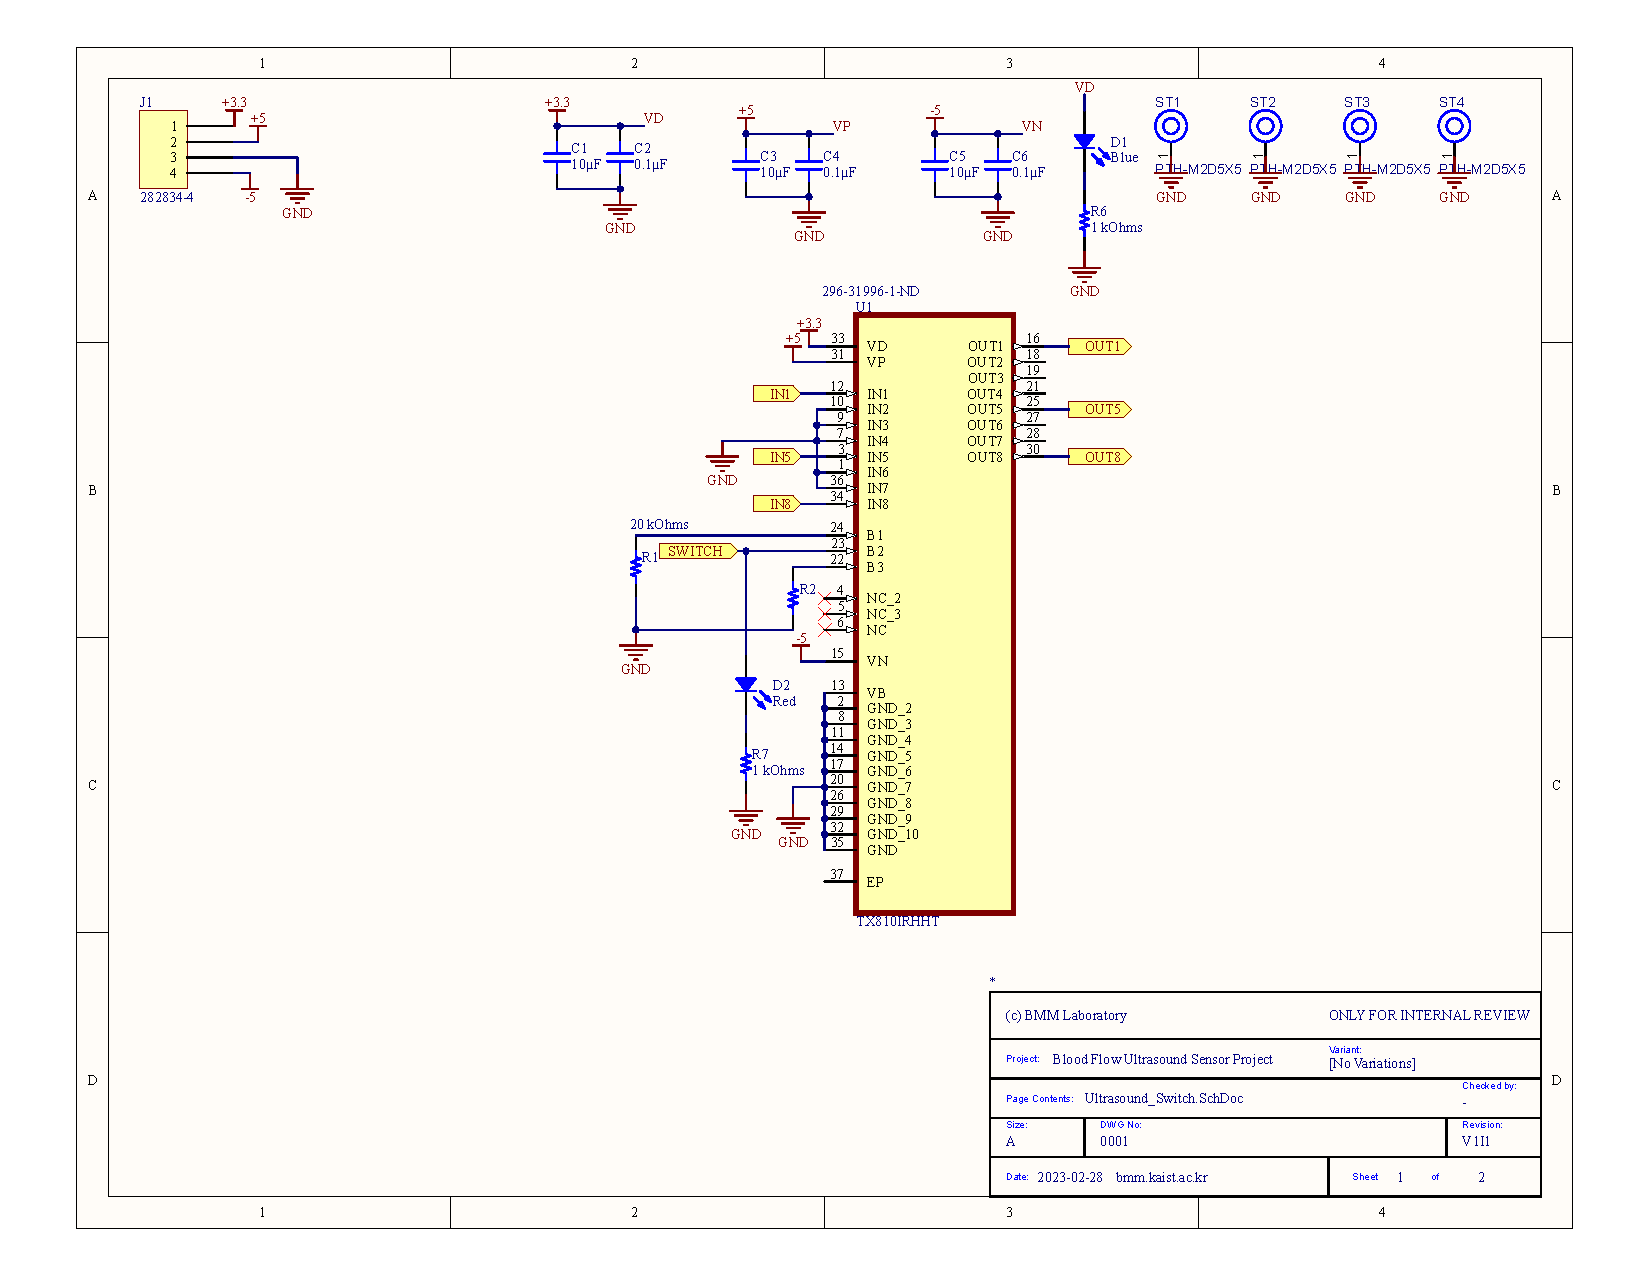
\includegraphics[width=20cm,height=28.7cm,keepaspectratio]{Figures/appendix/ultrasound_switch.pdf}
%		\caption{UltrasoundSwitch Schematic A}
%		\label{fig:appendix_ultrasoundswitch_a}
%	\end{figure}
%\end{landscape}
%\begin{landscape}
%	\begin{figure}[htbp]
%		\centering
%		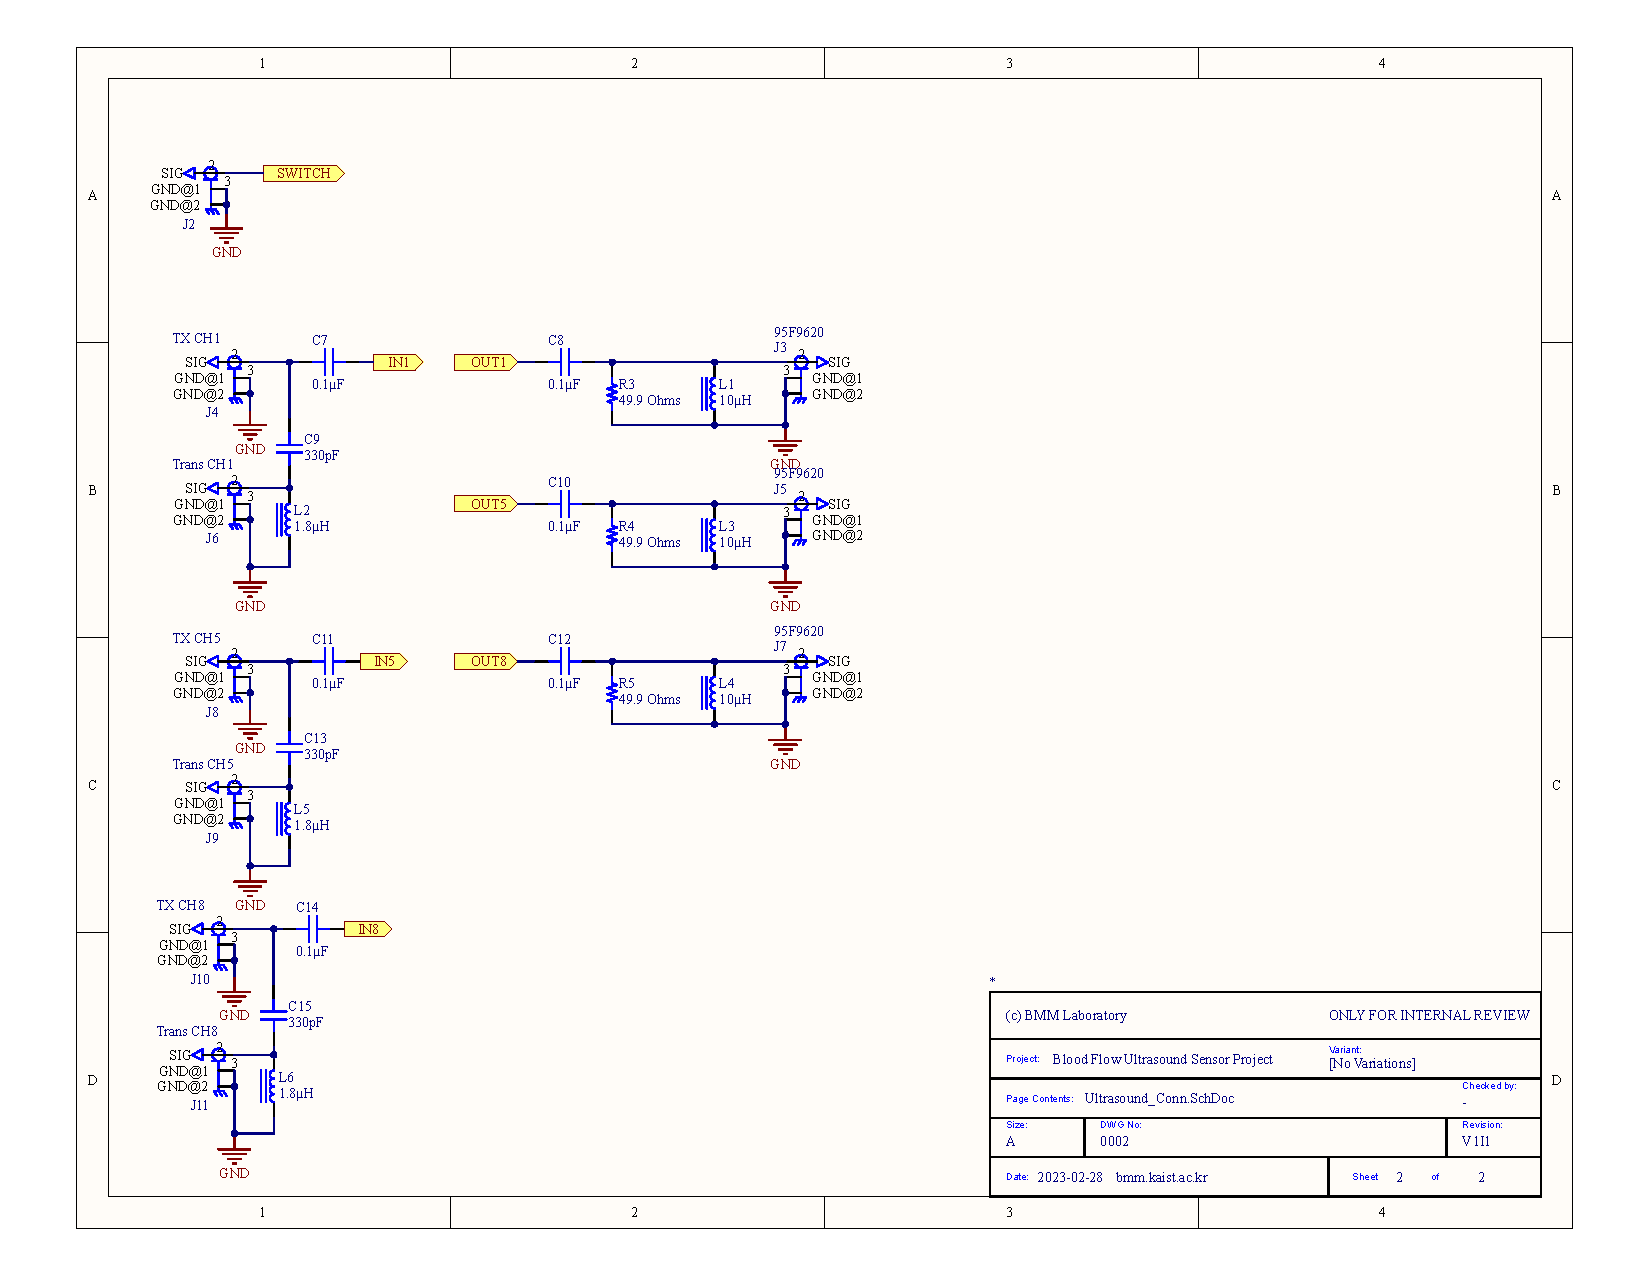
\includegraphics[width=20cm,height=28.7cm,keepaspectratio]{Figures/appendix/ultrasound_conn.pdf}
%		\caption{UltrasoundSwitch Schematic B}
%		\label{fig:appendix_ultrasoundswitch_b}
%	\end{figure}
%\end{landscape}
%\begin{landscape}
%	\begin{figure}[htbp]
%		\centering
%		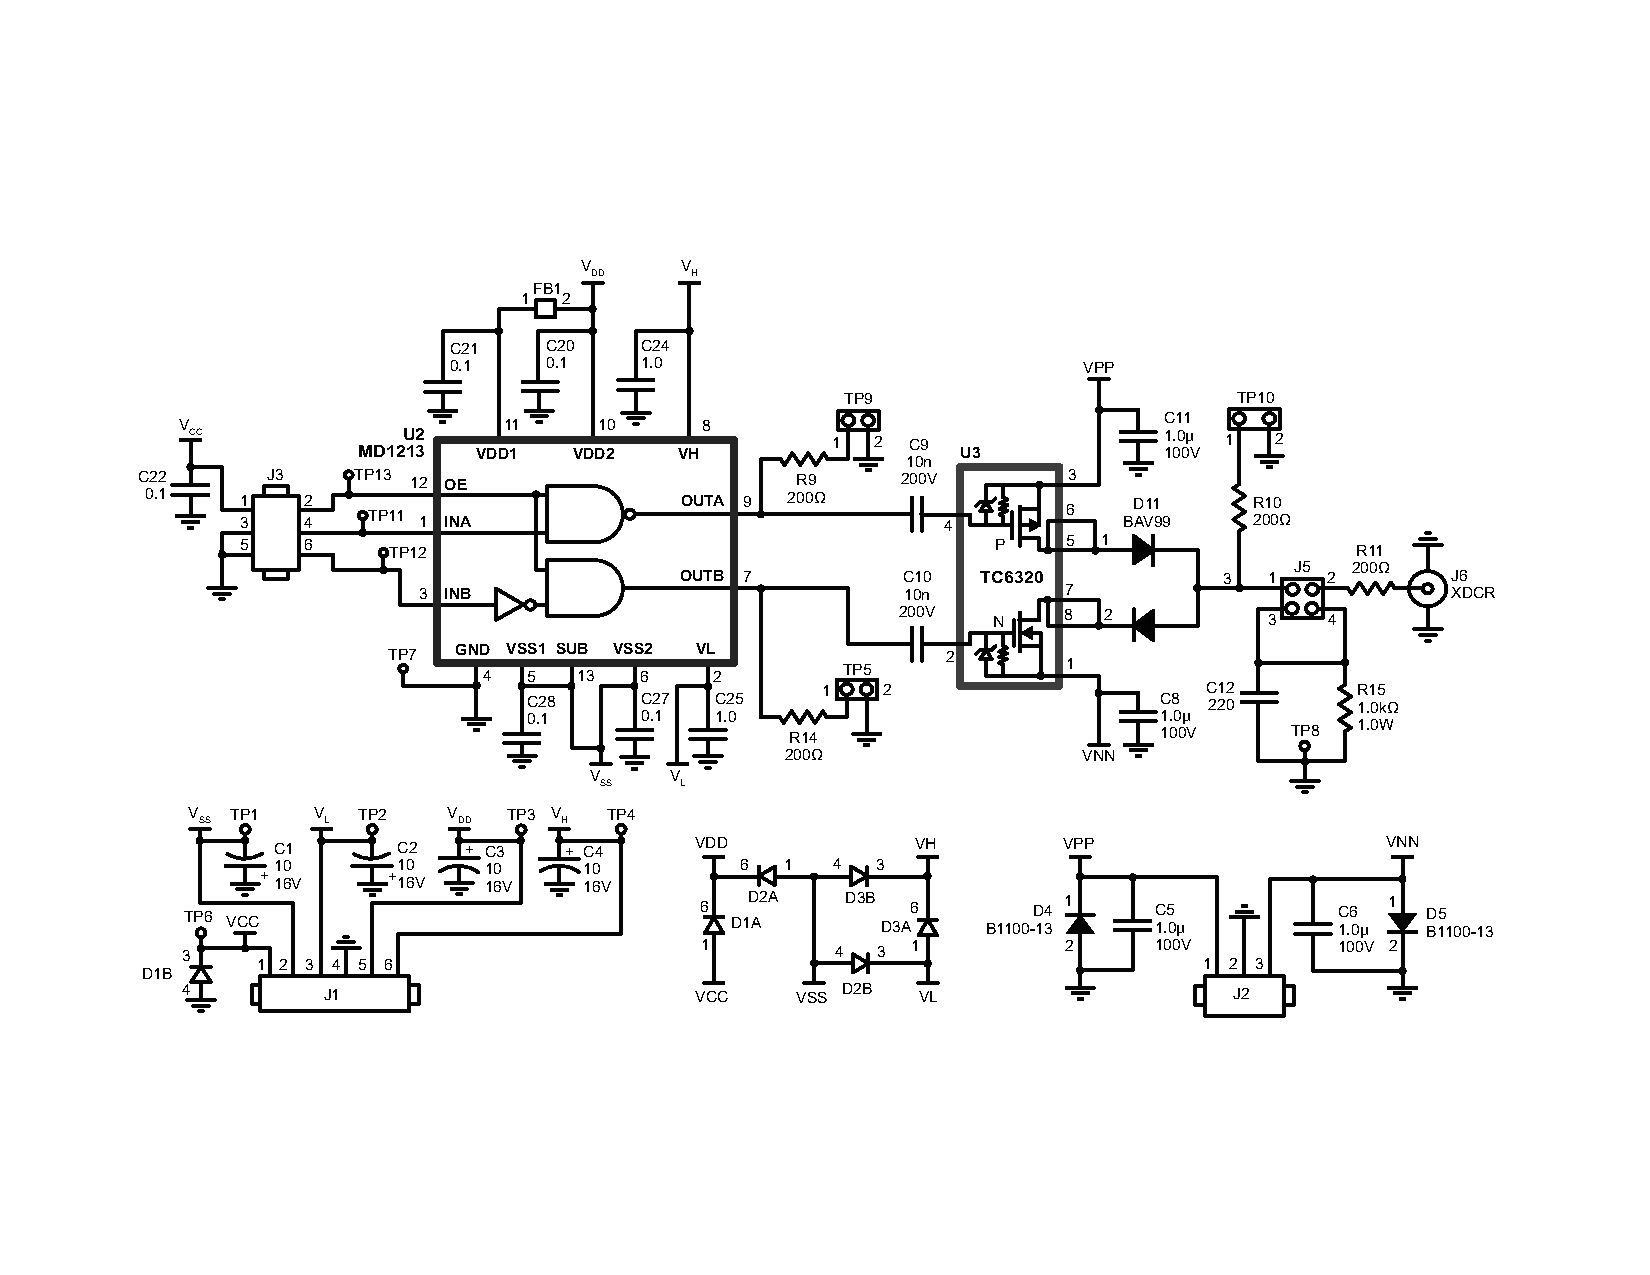
\includegraphics[width=20cm,height=28.7cm,keepaspectratio]{Figures/appendix/md1213db1_final.pdf}
%		\caption{MD1213DB1 Transmitter Schematic}
%		\label{fig:appendix_md1213db1}
%	\end{figure}
%\end{landscape}
%\begin{landscape}
%	\begin{figure}[htbp]
%		\centering
%		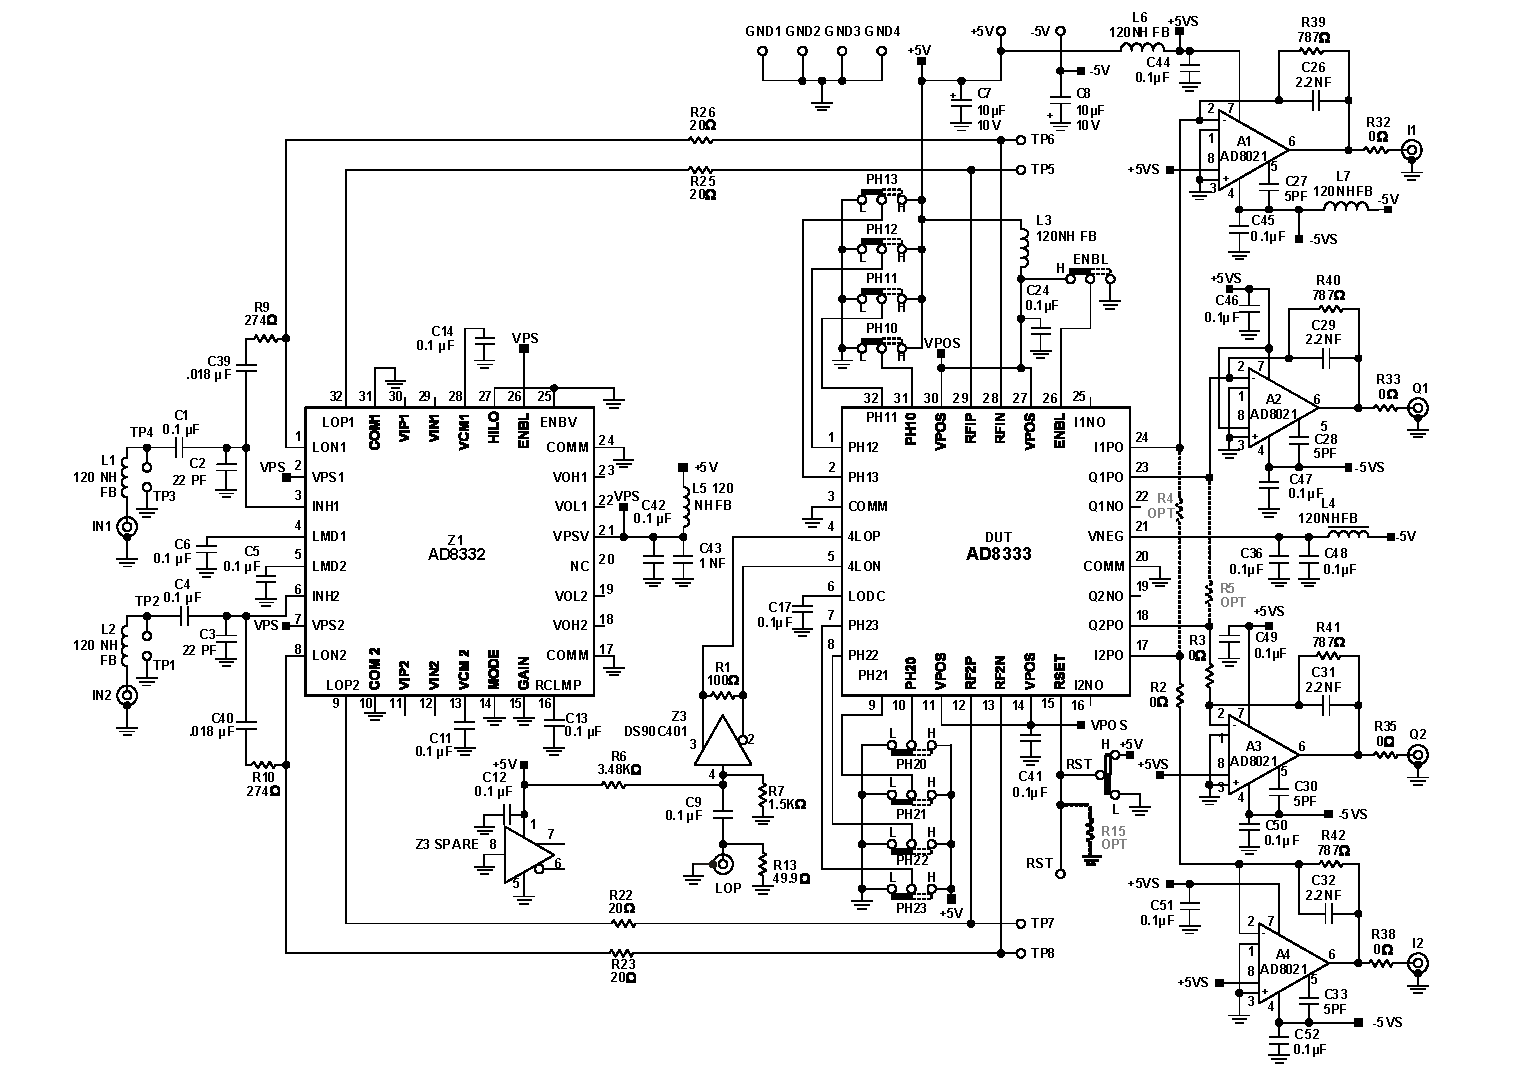
\includegraphics[width=20cm,height=28.7cm,keepaspectratio]{Figures/appendix/ad8333evalz.pdf}
%		\caption{AD8332 Preamplifier, AD8333 IQ Demodulator and Phase Shifter Schematic}
%		\label{fig:appendix_ad8333}
%	\end{figure}
%\end{landscape}
%\chapter{Circuit CAD Assembly Documentation}
%\begin{landscape}
%	\begin{figure}[htbp]
%		\centering
%		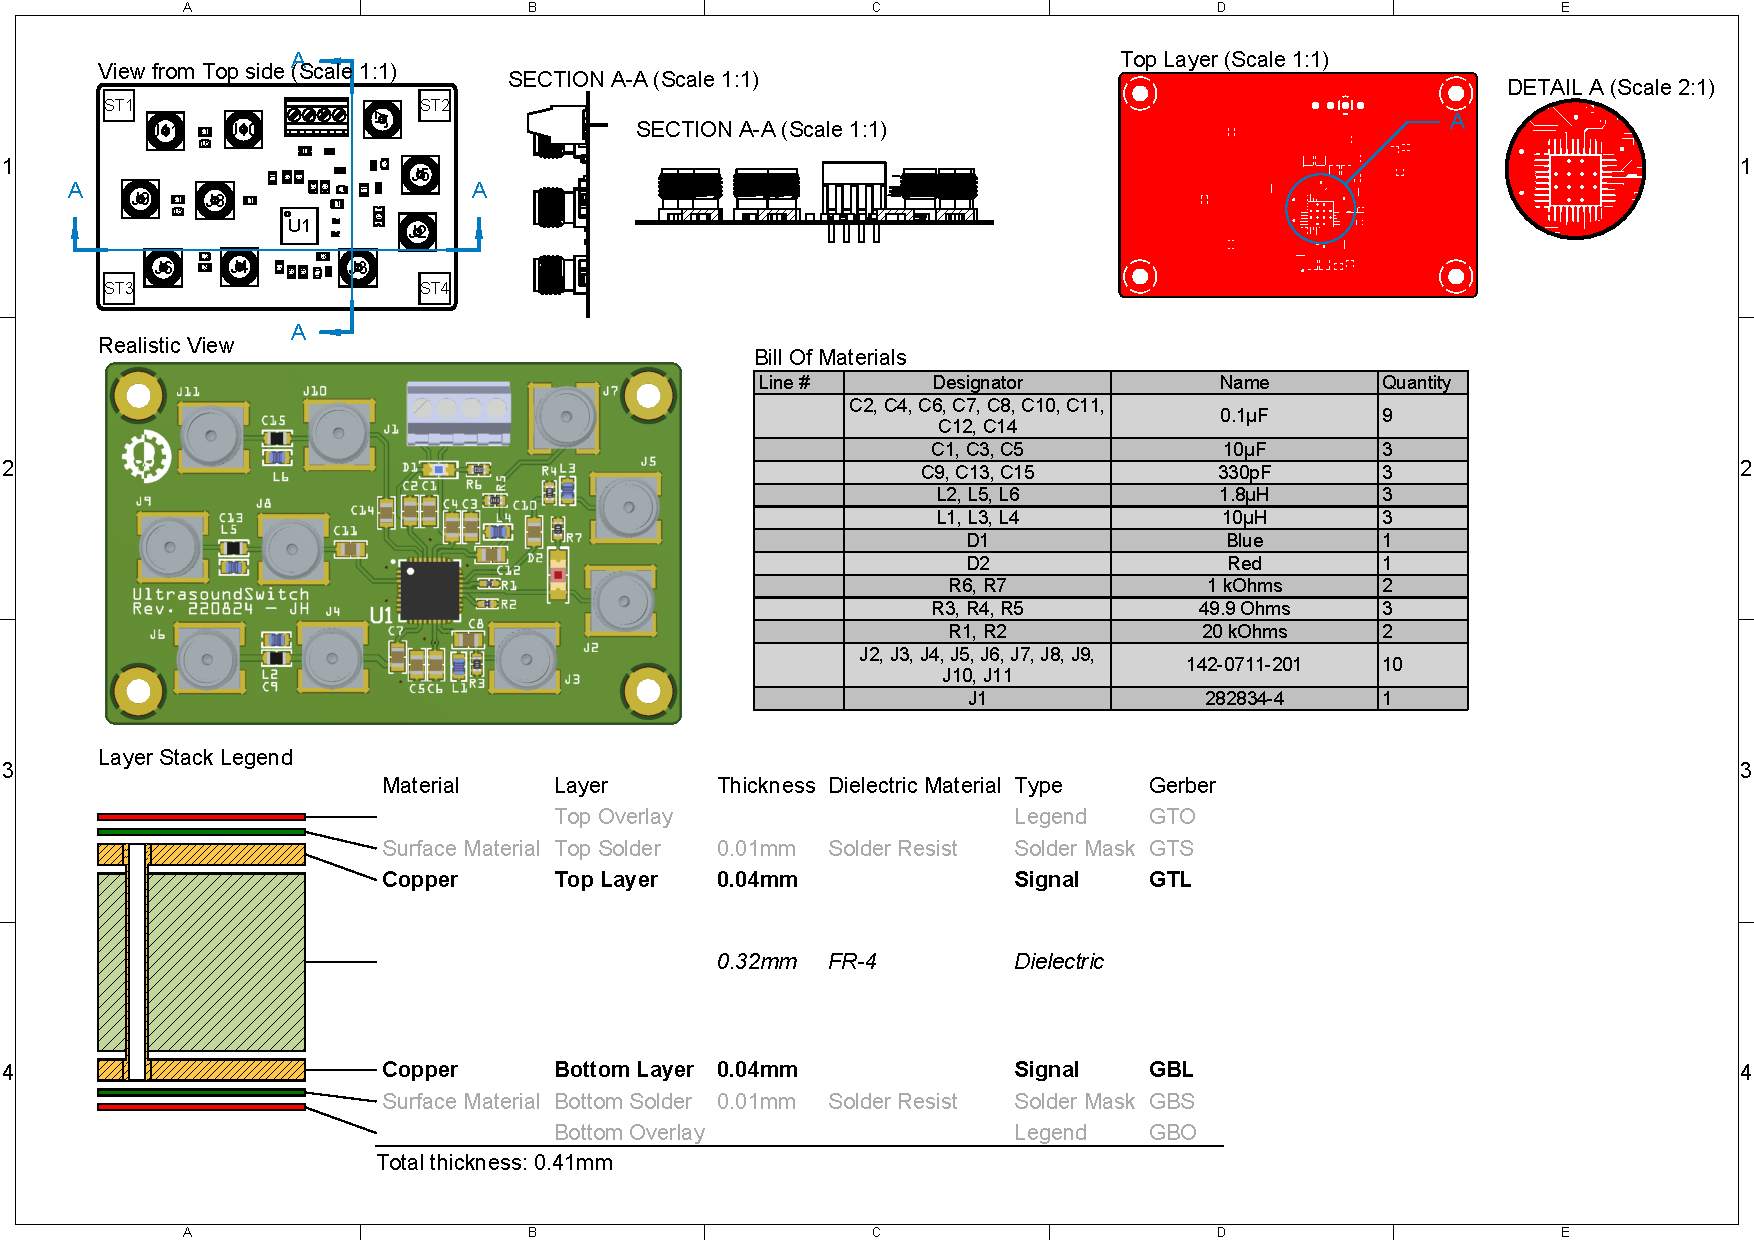
\includegraphics[width=20cm,height=28.7cm,keepaspectratio]{Figures/appendix/draftsman.pdf}
%		\caption{UltrasoundSwitch Assembly Information}
%		\label{fig:appendix_ultrasoundswitch_assembly}
%	\end{figure}
%\end{landscape}

%\chapter{Bill of Materials} \thispagestyle{main}
%
%	\begin{longtblr}[
%		%	theme=fancy,
%		caption = {Bill of Materials for the entire system},
%		entry={BOM},
%		label = {tab:bom}
%		]{
%			colspec = {lllll},
%			width = \linewidth,
%			rowhead = 1,
%%			hspan=minimal,
%			%vspan=minimal,
%		}
%		\toprule
%		{\textbf{Component}}
%		& {\textbf{Value}}
%		& {\textbf{Footprint}}
%		& {\textbf{Classification}}
%		& {\textbf{Description}}                              \\
%		\midrule
%		% table body
%		\SetCell[c=5]{c}{} Transmitter & & & & \\ \midrule
%		C1 & 1n & 0603 & X7R50V & Preamp \\
%		C13 & 1u & RAD-0.3in & Film 40V & Preamp \\
%		C14 & 1.5n & 0603 & X7R50V & PI controller \\
%		C15 & NC & 0603 & X7R50V & PI controller \\
%		C2,C3,C4 & 100n & 0603 & X7R16V & Decoupling \\
%		C5,C11 & 1u & 0603 & X5R6.3V & Decoupling \\
%		C6,C7 & 100n & 0805 & X7R50V & Decoupling \\
%		C8 & 1500u & RAD-0.3in & 63Vdc & Decoupling \\
%		P10 & 3-pin & Male & 250V & Controller bypass \\
%		P11,P12 & 10-pin & Female & 250V & InterPCB con. \\
%		P2,P3 & 1-pin header & Male & 250V & Measurements \\
%		P4,P5 & 2-way screw & NA & 300V 15A & Power,Output \\
%		P6 & 2-pin header & KK254 & 500V 4A & Audio in \\
%		P7 & 4-pin header & Female & 250V & 5V Power \\
%		P8,P9 & BNC & PCB & 500V & Audio in, Output \\
%		R2 & 16.2k & 0603 & 1\% & Preamp \\
%		R1,R3 & 2k & 0603 & 1\% & Preamp \\
%		R4,R7 & 4.75k & 0603 & 1\% & Voltage ref \\
%		R5 & 33.2k & 0603 & NA & PI controller \\
%		R6 & 0 (short) & 0603 & NA & PI controller \\
%		R9 & 0 (short) & 0603 & NA & PI controller \\
%		R10 & NC & 0603 & NA & PI controller \\
%		R8 & 2.49k & 0603 & 1\% & Voltage ref \\
%		U1 & OPA2365 & SOIC-8 & NA & Preamp, PI \\
%		U2 & TLV431A & SOT-23 & 1\% & Voltage ref \\ %\pagebreak
%		\SetCell[c=5]{c}{} Receiver & & & & \\ \midrule
%		C1,C11,C15 & 100n & 0603 & X7R16V & Gate driver \\
%		P1,P2 & 10-pin header & Male & 250V & InterPCB con. \\
%		C2,C16 & 150n & 0603 & X5R10V & Gate driver \\
%		C3,C10 & 100p & 0603 & NPO50V & Decoupling \\
%		L1,L2 & 1.768u & Radial & NA & Output filter \\
%		U1,U3 & LM5113 & WSON-10 & NA & Gate driver \\
%		R20 & 15m sense & 1210 & 1\% 1W & Output filter \\
%		R1,R6 & 500 & 3213 & NA & Gate driver \\
%		Q1,Q2,Q3,Q4 & BSZ097-N10NS5 & TSDSON-8 & NA & Power stage \\
%		R2,R5,R8,R10 & 5 & 0603 & 1\% & Gate driver \\
%		R4,R9 & 0 & 0603 & 1\% & Gate driver \\
%		D1,D2 & Diode & NA & 85V 0.25A & Gate driver \\
%		C5,C6,C9,C17 & 10u & 1210 & X7R50V & Decoupling \\
%		C12,C13,C14 & 680n & 1210 & X7R100V & Output filter \\
%		\SetCell[c=5]{c}{} Microcontroller & & & & \\ \midrule
%		C18,C20,C27 & 100n & 0603 & X7R16V & Decoupling \\
%		C28,C29 & 100n & 0603 & X7R16V & Decoupling \\
%		U6 & LT1999 & MSOP-8 & NA & Current acq. \\
%		U4 & AD8274 & MSOP-8 & NA & Volt acq. \\
%		U2 & LT1711 & MSOP-8 & NA & AIM \\
%		C4 & NC & 0603 & X7R16V & AIM \\
%		C7 & NC & 0603 & X7R16V & AIM \\
%		C8 & NC & 0603 & X7R16V & Cur. acq. \\
%		CA1 & 1.5n & 0603 & X7R50V & AIM \\
%		R14 & 8.66k & 0603 & 1\% & AIM \\
%		R18 & 16.2k & 0603 & 1\% & AIM \\
%		R23 & 1.5k & 0603 & 1\% & AIM \\
%		R3,R11 & 120k & 0603 & 1\% & Voltage acq. \\
%		RA1 & 2.2k & 0603 & 1\% & AIM \\
%		RA2 & 20k & 0603 & 1\% & AIM \\
%		RA3 & 2.74k & 0603 & 1\% & AIM \\
%		RA4 & 0 & 0603 & NA & AIM \\
%		\bottomrule
%	\end{longtblr}

\chapter{Instruments} \thispagestyle{main}
\begin{table}[ht]
	\centering
	\caption{List of instruments used for solder work}
	\label{tab:instruments_solder_work}
	\begin{tblr}[]{%
			colspec = {lll},
			row{1} = {guard, m, font=\small\bfseries},
		}
		\toprule
		Function & Manufacturer & Model \\ \midrule
		Visual inspection microscope & Leica & A60 \\
		Manual soldering & Weller & WX2 \\
		Heat gun & Thermaltronics & TMT-HA600-2 \\
		Solder paste & Chip Quik & SMD291AX250T3 \\
		Solder flux & Chip Quik & SMD291NL \\
		Reflow oven & Puhui & T-962A \\
		DMM & Fluke & 175 \\ \bottomrule
	\end{tblr}
\end{table}

\begin{table}[ht]
	\centering
	\caption{List of instruments used in experiments}
	\label{tab:instruments_hardware}
	\begin{tblr}[]{%
			colspec = {lll},
			row{1} = {guard, m, font=\small\bfseries},
		}
		\toprule
		Function & Manufacturer & Model \\
		\midrule
		DCPS 1 & RIGOL & DP832A 200W \\
		DCPS 2 & Keysight & E3631A 80W \\
		Function generator 1 & Keysight & 33500B \\
		Function generator 2 & Tektronix & AFG3102 \\
        DMM & Fluke & 175 \\
		Transducer (PZT) & HAGISONIC & M715-SB-S 204 \qty{5}{\mega\hertz} \\
		Transducer (CMUT) & BMM Creation & 6ch \qty{3.3}{\mega\hertz} C.F. \\
		RF Amplifier & Tomco & BT00100-AlphaS-CW \\
		Oscilloscope 1 & Keysight & DSO-X 2024A \\
		Oscilloscope 2 & Tektronix & MSO4054 \\
		Physiological simulator & CIRS & Doppler String Phantom 043A \\
		Vector Network Analyzer & TBD & TBD \\
	\end{tblr}
\end{table}
